\documentclass[11pt]{article}

\usepackage[utf8]{inputenc}
\usepackage[english]{babel}
\usepackage{hyperref}

\usepackage{amsmath}
\usepackage{physics}

\usepackage{graphicx}

\usepackage{listings}
\lstset{language=python}

\usepackage[style=nature]{biblatex}
\addbibresource{references.bib}

\title{Search and Task Allocation \\
    \small{Swarm Intelligence}}

\author{Sebastian G. Winther-Larsen}


\begin{document}
    
    \maketitle

    \section{Formalism}

    We define a search $A$ as an area bound by two points. Over the search area, 
    $n_T$ tasks $T$ are spawned at random positions. The tasks have a task capacity
    $T_c$ indicating how many agents $R$ are required to solve a task. The task is 
    solved immeadeately if $T_c$ agents are within the task radius $T_r$.
    The agents $R$ move randomly around the search area at a speed $R_v$. There are 
    $n_R$ agents. When an agent is inside the task radius $T_r$ of a task, the agents 
    will wat for other agents to complete the task. The agents can also call for 
    aid in solving a task. The communication distance $R_d$ determines how 
    far an agent can send a call for aid to another agent.

    The position of the agents are updated in a discrete Langevinian manner,
    \begin{equation}
        \label{eq:langevinian}
        r_{R, t+1} = r_{R, t} + N\left(a_R +  b_{R, t}\right),
    \end{equation}
    where $r_{R, t}$ is the position of agent $R$ at time $t$, $a_r$ is a 
    drift term, $b_{R, t}$ is a stochastic velocity term and $N$ is a normalising
    operator, ensuring equal velocity of all agents. The drift term is assigned 
    at the start of each simulation and the stochastic velocity term is updated 
    for each time step. The trend is added in order to make sure that the agents
    will venture away from their origin point, as the expected value of 
    a sum of equally distributed stochastic variables with mean zero will be 
    zero. That is, even though there is a likelihood for agents to evetually 
    cover the entire area, one would expect them to meander about the point 
    they were initially placed.

    In addition to walking randomly across the area, the agents have the 
    possiblity of calling other agents in the vicinity, if they are within 
    a communication distance $R_d$.

    \section{Implementation} 

    We implement a tool for visualising the problem described above in 
    PyGame~\cite{pygame}.
    The full implementation is available at \url{github.com/gregwinther/mas},
    and consists of three classes. Two of these, \lstinline!Task! and \lstinline!Agent!,
    both inherit from PyGame's \lstinline!Sprite! class. The last class,
    \lstinline!Simulation!, takes care of the game mechanics such as updating
    states and drawing the area with tasks and agents. Initialising and running 
    a particular game (simulation) can be done with very few lines. For example;
    \begin{lstlisting}
        simulation = Simulation(1000)
        simulation.cycles = 1000
        simulation.communicate = True
        simulation.write = True
        simulation.n_T = 3
        simulation.Tr = 50
        simulation.n_R = 10
        simulation.Tc = 3
        simulation.start()
    \end{lstlisting}
    A screenshot of this example is shown in \autoref{fig:sample_screenshot}.

    \begin{figure}
        \centering
        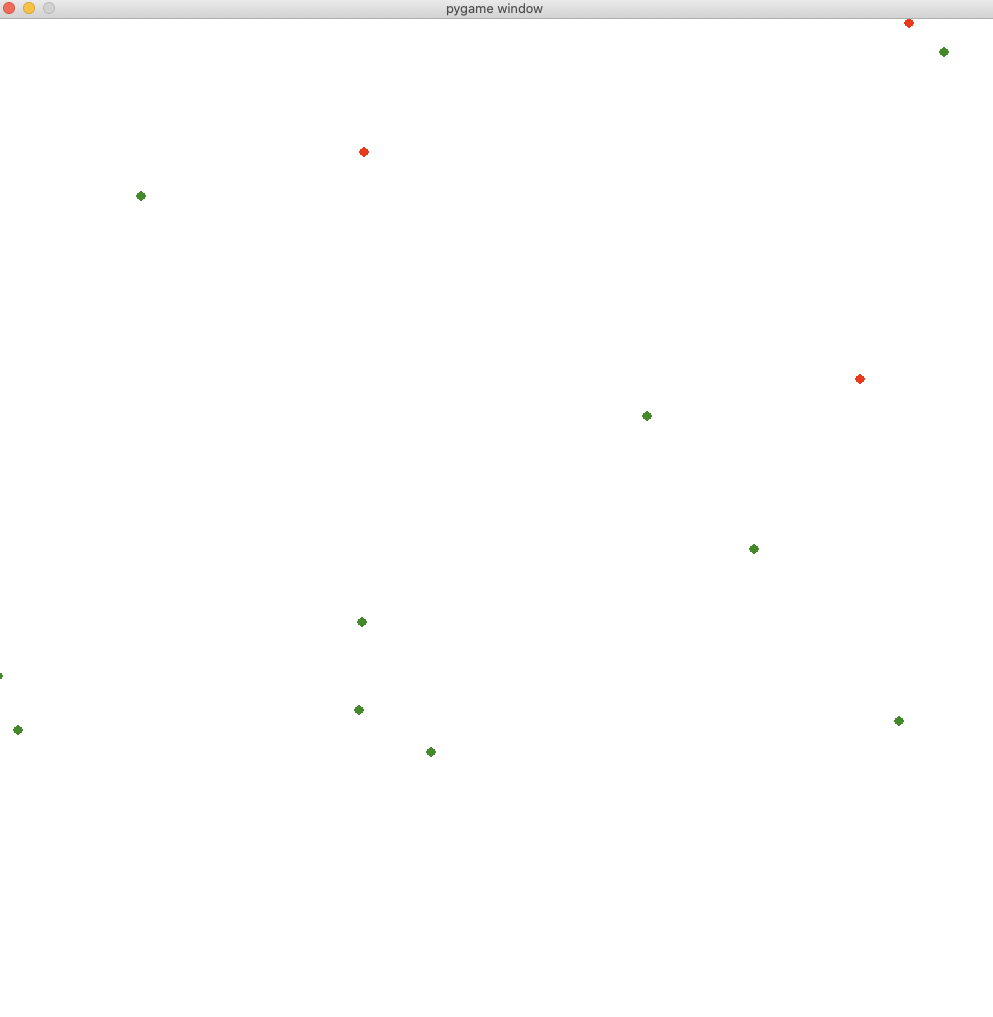
\includegraphics[width=0.8\textwidth]{figures/screenshot.png}
        \caption{\label{fig:sample_screenshot}
            Sample screenshot of a simulation with $n_T=3$ and $n_R=10$.
            The green dots are agents $R$, and the red 
            dots are tasks $T$. 
        }
    \end{figure}

    The most important methods of the \lstinline!Task! and \lstinline!Agent!
    classes is the \lstinline!update()! method, which is called for 
    each iteration of the game. For a Task, this method is 
    quite simple. It simple checks if there are enough agents within the 
    task radius $T_r$ to complete the task, if so the task sprite is killed.
    
    The \lstinline!update()! method for agents is more subtle. Firstly, it has to 
    update the positions of the agents according to \autoref{eq:langevinian}. 
    This is done by generating a random movement step, or finite difference velocity,
    which is added to the trend and then normalised to have lenght equal to $R_v$.

    Since it is possible for an agent to wander outside the area, we take care of 
    the boundaries in the following manner. When a moving agent hits one of the
    boundaries of the area, the trend unit vector which is perpendicular to 
    the boundary line is reversed. This has the effect of ``soft bounce'' 
    off the boundary.

    More than the mere movement of the agents, it is possible for them to be in
    different states. They may be \emph{searching}, \emph{tasked} or \emph{called}.
    The default state, \emph{searching}, is what we just described above. Whenever
    an agent is within the task radius $T_r$ of a task $T$ its state will change 
    to \emph{tasked}. If the task capacity $T_c$ required more agents than the
    one(s) present, the agent will stay put until enough agents arrive at the 
    task to help. With the mechanic enabled, an agent may also be \emph{called}
    if it is within the communication distance $R_d$ of another agent. The agent 
    will then move at speed towards the position of the signalling agent. All of the 
    transitions between agent states are handled within the main game loop 
    of the \lstinline!Simulation! class.

    \section{Results}

    \section{Discussion}
    

    \printbibliography

\end{document}